\documentclass[8pt,a4paper,compress]{beamer}

\usepackage{/home/siyer/lib/slides}

\title{Binary Search Trees}
\date{}

\begin{document}
\begin{frame}
\vfill
\titlepage
\end{frame}

\begin{frame}
\frametitle{Outline}
\tableofcontents
\end{frame}

\section{What is a Binary Search Tree (BST)?}
\begin{frame}[fragile]
\pause

A binary tree is either empty or a node with a key (and associated value) and links (left and right) to two disjoint binary subtrees

\pause
\bigskip

A binary tree is in symmetric order if each node's key is larger than all keys in its left subtree and smaller than all keys in its right subtree

\pause
\bigskip

A binary search tree (BST) is a binary tree in symmetric order

\smallskip

\begin{center}
\visible<4->{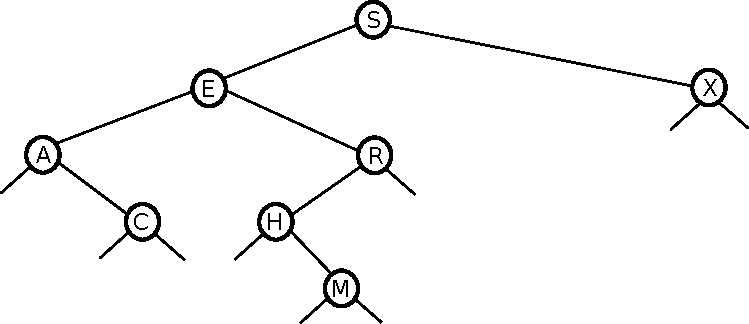
\includegraphics[scale=0.6]{./figures/bst.pdf}}
\end{center}
\end{frame}

\begin{frame}[fragile]
\pause

A BST representation in Java is a reference to a root node, which is composed of five fields: a key, a value, a reference to the left subtree, a reference to the right subtree, and the number of nodes in the subtree

\pause

\begin{lstlisting}[language=Java]
private class Node {
    private Key key; 
    private Value val; 
    private Node left, right; 
    private int N;

    public Node(Key key, Value val, int N) {
        this.key = key;
        this.val = val;
        this.N = N;
    }
}
\end{lstlisting}
\end{frame}

\section{Implementation of the Ordered Symbol Table API Using a BST}
\begin{frame}[fragile]
\pause

Basic operations

\begin{lstlisting}[language=Java]
package edu.princeton.cs.algs4;

import java.util.NoSuchElementException;

public class BST<Key extends Comparable<Key>, Value> {
    private Node root;
    
    public BST() {}
    
    public boolean isEmpty() { return size() == 0; }

    public int size() { return size(root); }

    private int size(Node x) {
        if (x == null) { return 0; }
        else return x.N;
    }

    public Value get(Key key) { return get(root, key); }

    private Value get(Node x, Key key) {
        if (x == null) { return null; }
        int cmp = key.compareTo(x.key);
        if      (cmp < 0) { return get(x.left, key); }
        else if (cmp > 0) { return get(x.right, key); }
        else              { return x.val; }
    }

    public boolean contains(Key key) { return get(key) != null; }
\end{lstlisting}
\end{frame}

\begin{frame}[fragile]
\pause

\begin{lstlisting}[language=Java]
    public void put(Key key, Value val) {
        if (val == null) { delete(key); return; }
        root = put(root, key, val);
    }

    private Node put(Node x, Key key, Value val) {
        if (x == null) { return new Node(key, val, 1); }
        int cmp = key.compareTo(x.key);
        if      (cmp < 0) { x.left  = put(x.left,  key, val); }
        else if (cmp > 0) { x.right = put(x.right, key, val); }
        else              { x.val   = val; }
        x.N = 1 + size(x.left) + size(x.right);
        return x;
    }
}
\end{lstlisting}
\end{frame}

\begin{frame}[fragile]
\pause

Tree shape depends on order of insertion

\begin{minipage}{100pt}
\begin{center}
\visible<2->{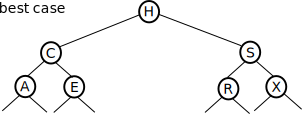
\includegraphics[scale=0.4]{{./figures/bst_possibility1}.pdf}}
\end{center}
\end{minipage}%
\begin{minipage}{140pt}
\begin{center}
\visible<2->{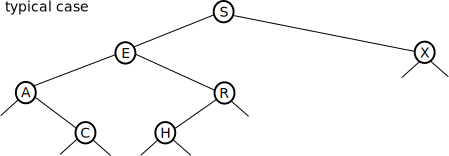
\includegraphics[scale=0.4]{{./figures/bst_possibility2}.pdf}}
\end{center}
\end{minipage}%
\begin{minipage}{50pt}
\begin{center}
\visible<2->{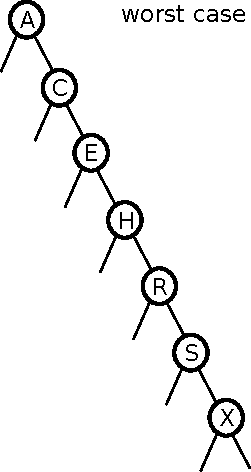
\includegraphics[scale=0.4]{{./figures/bst_possibility3}.pdf}}
\end{center}
\end{minipage}

\pause
\bigskip

Number of comparisons for search/insert is equal to 1 + depth of node

\pause
\bigskip

If $N$ distinct keys are inserted into a BST in random order,
the expected number of comparisons for a search/insert is $\sim 2\ln N$
\end{frame}

\begin{frame}[fragile]
\pause

Typical BST, built from 256 random keys

\begin{center}
\visible<2->{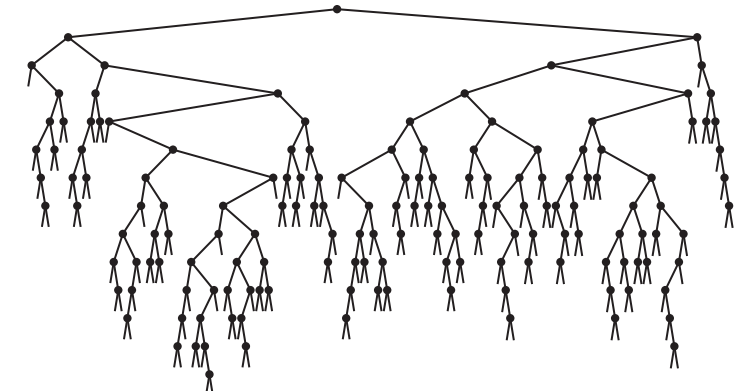
\includegraphics[scale=0.4]{{./figures/typical_bst}.png}}
\end{center}
\end{frame}

\begin{frame}[fragile]
\pause

Minimum and maximum

\smallskip

\begin{center}
\visible<2->{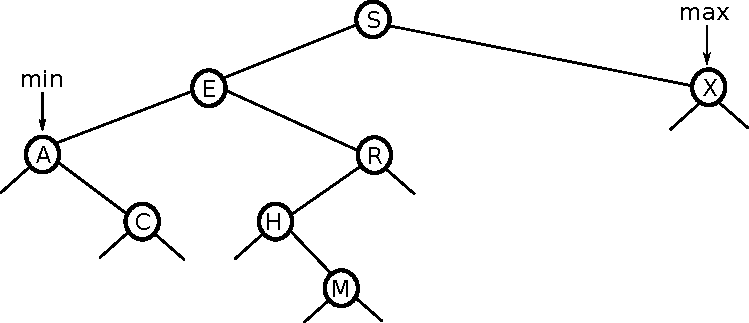
\includegraphics[scale=0.4]{{./figures/bst_min_max}.pdf}}
\end{center}

\pause

\begin{lstlisting}[language=Java]
    public Key min() {
        if (isEmpty()) { return null; }
        return min(root).key;
    } 

    private Node min(Node x) { 
        if (x.left == null) { return x; }
        else                { return min(x.left); } 
    } 

    public Key max() {
        if (isEmpty()) { return null; }
        return max(root).key;
    } 

    private Node max(Node x) { 
        if (x.right == null) { return x; } 
        else                 { return max(x.right); } 
    } 
\end{lstlisting}
\end{frame}

\begin{frame}[fragile]
\pause

Floor and ceiling

\begin{center}
\visible<2->{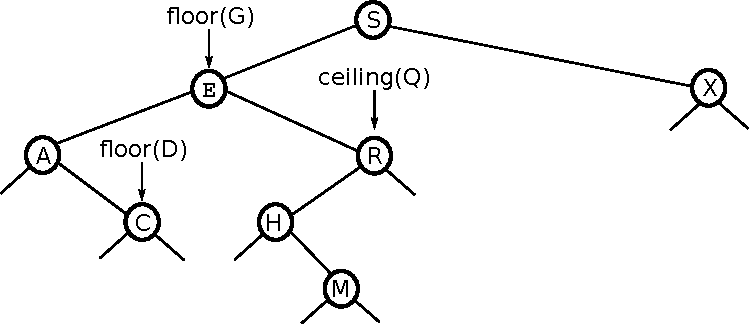
\includegraphics[scale=0.4]{{./figures/bst_floor_ceil}.pdf}}
\end{center}

\smallskip

Computing the floor of key $k$
\begin{itemize}
\item Case 1 ($k$ equals the key in the node): the floor of $k$ is $k$

\item Case 2 ($k$ is less than the key in the node): the floor of $k$ is in the left subtree

\item Case 3 ($k$ is greater than the key in the node): the floor of $k$ is in the right subtree if there is any key $\leq k$ in there; otherwise, it is the key in the node
\end{itemize}

\pause

\begin{lstlisting}[language=Java]
    public Key floor(Key key) {
        Node x = floor(root, key);
        if (x == null) { return null; }
        else           { return x.key; }
    } 

    private Node floor(Node x, Key key) {
        if (x == null) { return null; }
        int cmp = key.compareTo(x.key);
        if (cmp == 0) { return x; }
        if (cmp <  0) { return floor(x.left, key); }
        Node t = floor(x.right, key); 
        if (t != null) { return t; }
        else           { return x; } 
    } 
\end{lstlisting}
\end{frame}

\begin{frame}[fragile]
\pause

Computing the ceiling of key $k$
\begin{itemize}
\item Case 1 ($k$ equals the key in the node): the ceiling of $k$ is $k$

\item Case 2 ($k$ is greater than the key in the node): the ceiling of $k$ is in the right subtree

\item Case 3 ($k$ is less than the key in the node): the ceiling of $k$ is in the left subtree if there is any key $\geq k$ in there; otherwise, it is the key in the node
\end{itemize}

\pause

\begin{lstlisting}[language=Java]
    public Key ceiling(Key key) {
        Node x = ceiling(root, key);
        if (x == null) { return null; }
        else           { return x.key; }
    }

    private Node ceiling(Node x, Key key) {
        if (x == null) { return null; }
        int cmp = key.compareTo(x.key);
        if (cmp == 0) { return x; }
        if (cmp > 0)  { return ceiling(x.right, key); }
        Node t = ceiling(x.left, key); 
        if (t != null) { return t; }
        else           { return x; }
    } 
\end{lstlisting}
\end{frame}

\begin{frame}[fragile]
\pause

Rank and selection

\begin{center}
\visible<2->{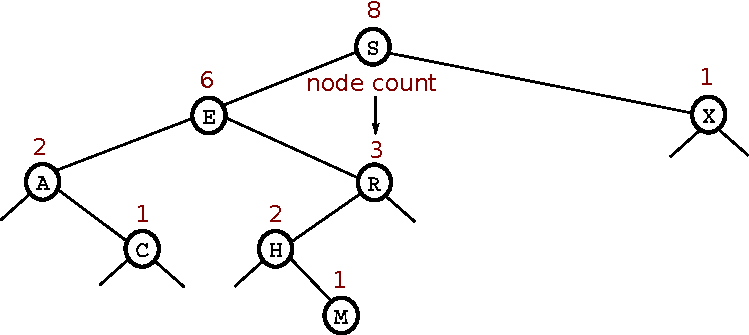
\includegraphics[scale=0.35]{{./figures/bst_rank_select}.pdf}}
\end{center}

\pause

\begin{lstlisting}[language=Java]
    public int rank(Key key) { return rank(key, root); } 

    private int rank(Key key, Node x) {
        if (x == null) { return 0; }
        int cmp = key.compareTo(x.key); 
        if      (cmp < 0) { return rank(key, x.left); }
        else if (cmp > 0) { return 1 + size(x.left) + rank(key, x.right); }
        else              { return size(x.left); }
    } 

    public Key select(int k) {
        if (k < 0 || k >= size()) { return null; }
        Node x = select(root, k);
        return x.key;
    }

    private Node select(Node x, int k) {
        if (x == null) { return null; } 
        int t = size(x.left); 
        if      (t > k) { return select(x.left,  k); }
        else if (t < k) { return select(x.right, k - t - 1); } 
        else            { return x; }
    } 
\end{lstlisting}
\end{frame}

\begin{frame}[fragile]
\pause

Range count and range search
\begin{lstlisting}[language=Java]
    public int size(Key lo, Key hi) {
        if (lo.compareTo(hi) > 0) { return 0; }
        if (contains(hi)) { return rank(hi) - rank(lo) + 1; }
        else              { return rank(hi) - rank(lo); }
    }

    public Iterable<Key> keys() {
        return keys(min(), max());
    }

    public Iterable<Key> keys(Key lo, Key hi) {
        Queue<Key> queue = new Queue<Key>();
        keys(root, queue, lo, hi);
        return queue;
    } 

    private void keys(Node x, Queue<Key> queue, Key lo, Key hi) { 
        if (x == null) { return; }
        int cmplo = lo.compareTo(x.key); 
        int cmphi = hi.compareTo(x.key); 
        if (cmplo < 0) { keys(x.left, queue, lo, hi); } 
        if (cmplo <= 0 && cmphi >= 0) { queue.enqueue(x.key); }
        if (cmphi > 0) { keys(x.right, queue, lo, hi); }
    } 
\end{lstlisting}
\end{frame}

\begin{frame}[fragile]
\pause

Deletion: to delete the minimum (maximum) key
\begin{itemize}
\item Go left (right) until you find a node with null left (right) link
\item Replace that node by its right (left) link
\item Update subtree counts
\end{itemize}

\pause

\begin{lstlisting}[language=Java]
    public void deleteMin() {
        if (isEmpty()) { throw new NoSuchElementException(); }
        root = deleteMin(root);
    }

    private Node deleteMin(Node x) {
        if (x.left == null) { return x.right; }
        x.left = deleteMin(x.left);
        x.N = size(x.left) + size(x.right) + 1; 
        return x;
    }

    public void deleteMax() {
        if (isEmpty()) { throw new NoSuchElementException(); }
        root = deleteMax(root);
    }

    private Node deleteMax(Node x) {
        if (x.right == null) { return x.left; }
        x.right = deleteMax(x.right);
        x.N = size(x.left) + size(x.right) + 1;
        return x;
    }   
\end{lstlisting}
\end{frame}

\begin{frame}[fragile]
\pause

\begin{minipage}{200pt}
Deletion: to delete a node with key $k$ (Hibbard deletion), search for the node $t$ containing key $k$
\begin{itemize}
\item Case 1 (0 children): delete $t$ by setting parent link to null

\item Case 2 (1 child): delete $t$ by replacing parent link

\item Case 3 (2 children): find successor $x$ of $t$ ($x$ has no left child); delete the minimum in $t$'s right subtree; and put $x$ in $t$'s spot
\end{itemize}
and update subtree counts
\end{minipage}%
\begin{minipage}{100pt}
\begin{center}
\visible<2->{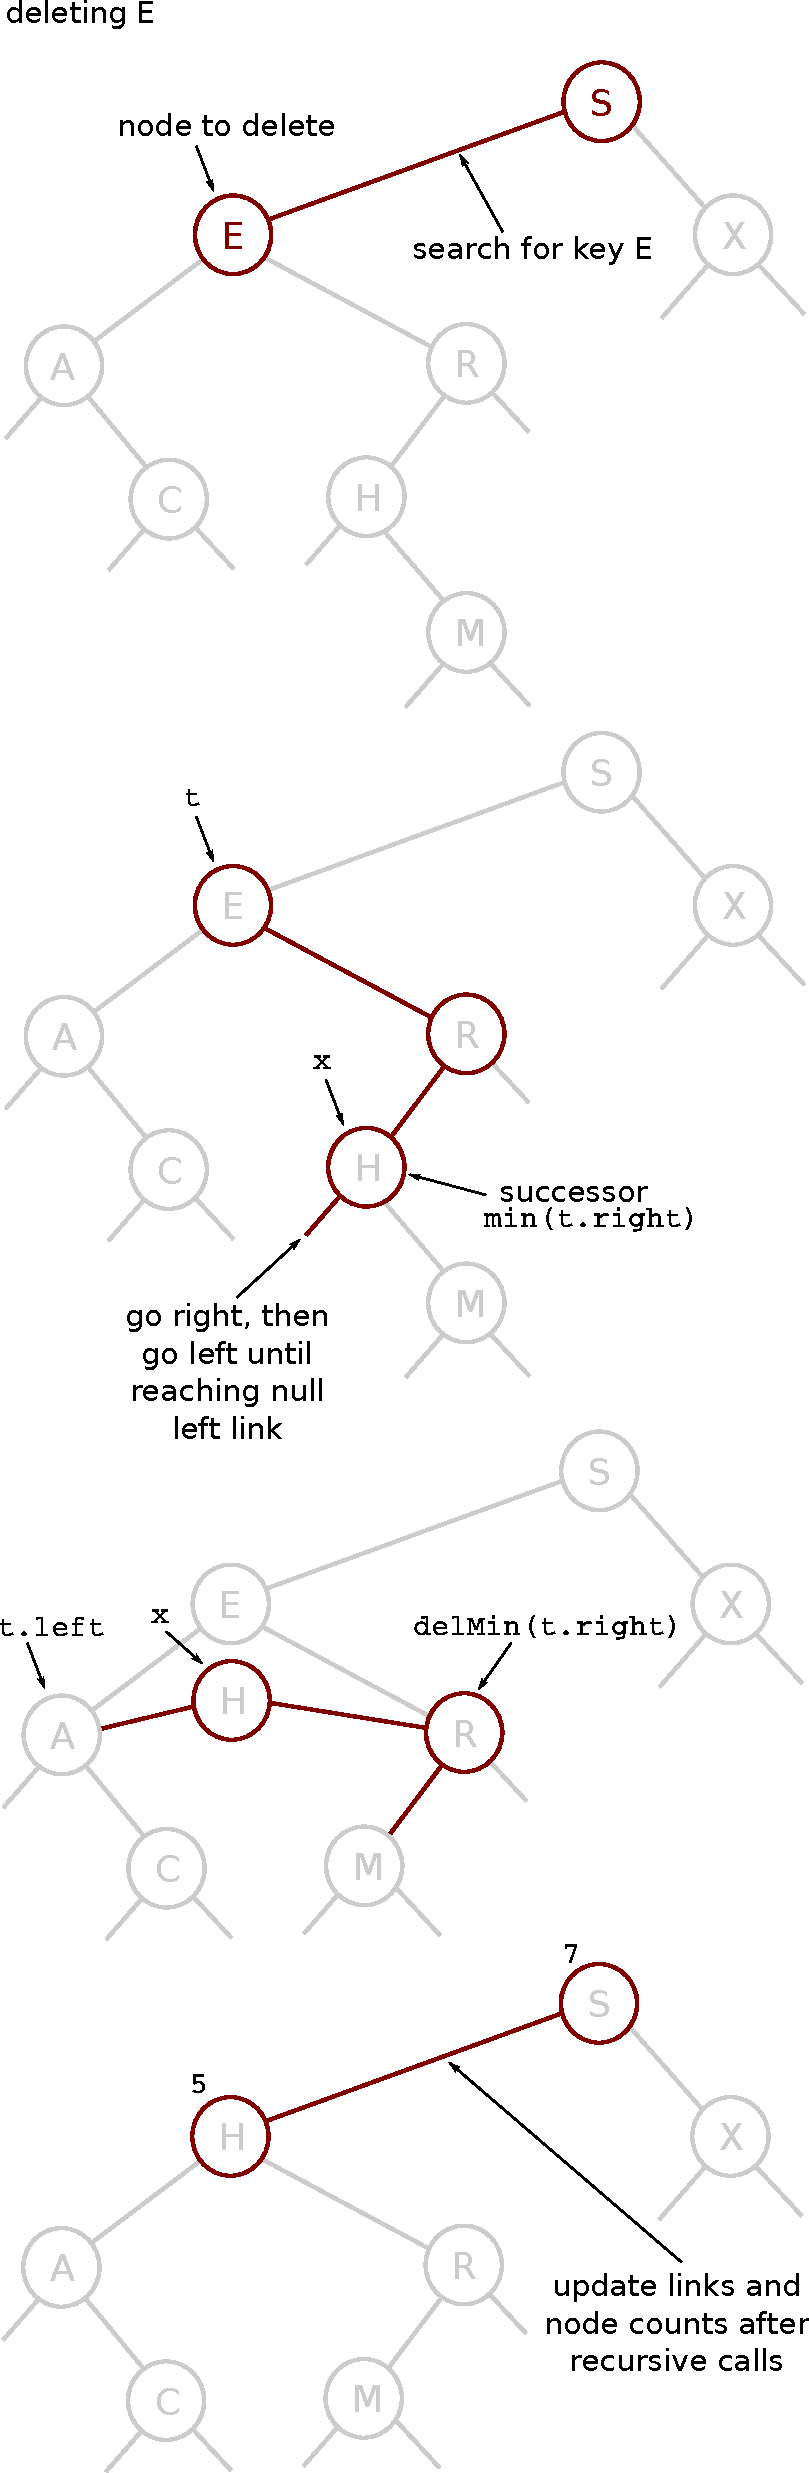
\includegraphics[scale=0.215]{./figures/bst_delete.pdf}}
\end{center}
\end{minipage}
\end{frame}

\begin{frame}[fragile]
\pause

\begin{lstlisting}[language=Java]
    public void delete(Key key) {
        root = delete(root, key);
    }

    private Node delete(Node x, Key key) {
        if (x == null) { return null; }
        int cmp = key.compareTo(x.key);
        if      (cmp < 0) { x.left  = delete(x.left,  key); }
        else if (cmp > 0) { x.right = delete(x.right, key); }
        else { 
            if (x.right == null) { return x.left; }
            if (x.left  == null) { return x.right; }
            Node t = x;
            x = min(t.right);
            x.right = deleteMin(t.right);
            x.left = t.left;
        } 
        x.N = size(x.left) + size(x.right) + 1;
        return x;
    } 
\end{lstlisting}
\end{frame}

\section{Binary Tree Traversal}
\begin{frame}[fragile]
\pause

Pre-order traversal
\begin{lstlisting}[language=Java]
public void preorder() { preorder(root); }

private void preorder(Node x) {
    if (x == null) { return; }
    process(x);
    preorder(x.left);
    preorder(x.right);
}
\end{lstlisting}

\pause
\bigskip

In-order traversal
\begin{lstlisting}[language=Java]
public void inorder() { inorder(root); }

private void inorder(Node x) {
    if (x == null) { return; }
    inorder(x.left);
    process(x);
    inorder(x.right);
}
\end{lstlisting}

\pause
\bigskip

Post-order traversal
\begin{lstlisting}[language=Java]
public void postorder() { postorder(root); }

private void postorder(Node x) {
    if (x == null) { return; }
    postorder(x.left);
    postorder(x.right);
    process(x);
}
\end{lstlisting}

\pause
\bigskip

In-order traversal of a BST processes keys in ascending order
\end{frame}

\begin{frame}[fragile]
\pause

For example, let \lstinline{T} denote the following BST
\begin{center}
\visible<2->{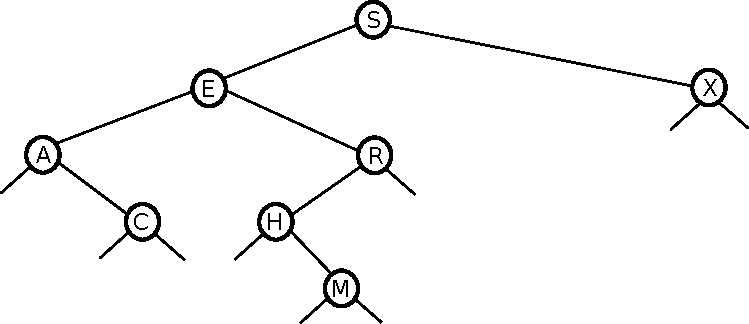
\includegraphics[scale=0.6]{./figures/bst.pdf}}
\end{center}

\pause
\bigskip

Then, the calls \lstinline{preorder(T)}, \lstinline{inorder(T)}, and \lstinline{postorder(T)} will process the tree in the following orders

\begin{center}
\lstinline{S    E    A    C    R    H    M    X}

\bigskip

\lstinline{A    C    E    H    M    R    S    X}

\bigskip

\lstinline{C    A    M    H    R    E    X    S}
\end{center}
\end{frame}

\section{Performance Characteristics}
\begin{frame}[fragile]
\pause

Symbol table operations summary
\begin{center}
\begin{tabular}{cccc}
operation & unordered linked list & ordered array & BST \\ \hline \\
search & $N$ & $\lg N$ & $h^\dagger$ \\
insert & $N$ & $N$ & $h$ \\
delete & $N$ & $N$ & $N^{\dagger\dagger}$ \\
min/max & - & 1 & $h$ \\
floor/ceiling & - & $\lg N$ & $h$\\
rank & - & $\lg N$ & $h$ \\
select & - & 1 & $h$ \\
ordered iteration & - & $N$ & $N$ 
\end{tabular} 

\bigskip

\tiny $\dagger$ $h$ is the height of BST, proportional to $\lg N$ if keys inserted in random order

$\dagger\dagger$ $\sqrt{N}$ in the average case; other operations also become $\sqrt{N}$ if deletions are allowed
\end{center}
\end{frame}
\end{document}
